\documentclass[12pt,a4paper]{article}

% Essential packages
\usepackage[utf8]{inputenc}
\usepackage[T1]{fontenc}
\usepackage[english]{babel} 
\usepackage{graphicx}
\usepackage{float}
\usepackage{hyperref}
\usepackage{booktabs}
\usepackage{array}
\usepackage{geometry}
\usepackage{amsmath}
\usepackage{amssymb}
\usepackage{xcolor}
\usepackage{longtable}
\usepackage{enumitem}

\usepackage{tikz}
\usetikzlibrary{shapes.geometric, arrows.meta, positioning, fit, backgrounds}


\geometry{left=2.5cm,right=2.5cm,top=3cm,bottom=3cm}


\hypersetup{
    colorlinks=true,
    linkcolor=blue,
    urlcolor=blue,
    citecolor=black
}

\begin{document}

% ==========================================
% TITLE PAGE
% ==========================================
\begin{titlepage}
    \centering
    \vspace*{1cm}
    {\Large \textbf{Universidad Distrital Francisco José de Caldas}} \\
    \vspace{0.4cm}
    {\large Faculty of Engineering \\ Systems Engineering Program} \\
    \vspace{2.5cm}
    {\Huge \textbf{Computational Simulation and System Validation Report}} \\
    \vspace{0.5cm}
    {\Large \textbf{Workshop 4: Discrete-Event Modeling, Complexity, and Chaos Analysis}} \\
    \vspace{2cm}
    \textbf{Authors (Engineering Team):} \\
    Omar Yesid Fonseca López (\texttt{oyfonsecal@udistrital.edu.co}) \\
    Daniel Felipe Barrera Suárez (\texttt{dfbarreras@udistrital.edu.co}) \\
    Daniel Mateo Ballesteros Molina (\texttt{dmballesterosm@udistrital.edu.co}) \\
    Dania Lizeth Guzmán Triviño (\texttt{dlguzmant@udistrital.edu.co}) \\
    \vfill
    \textbf{Course:} Systems Analysis \& Design \\
    \textbf{Professor:} Eng. Carlos Andrés Sierra, M.Sc. \\
    \vspace{1cm}
    Bogotá, Colombia \\
    2026
\end{titlepage}

\pagenumbering{roman}

% ==========================================
% ABSTRACT
% ==========================================
\begin{abstract}
This document presents the consolidation of \textbf{Workshop 4} for the \textbf{Smart Campus Energy Management System} project at the Sabio Caldas Campus. Building upon the systems analysis from Workshop 1 and the software architecture decisions in the user-space from Workshops 2 and 3, this report implements and validates a discrete-event computational model in Python. The simulation recreates a 12-hour stochastic operational cycle for a cluster of 20 workstations, injecting human behavioral factors (80\% probability of manual shutdown neglect) and technical complexity (15\% high computational load peaks). 

Empirical results conclusively validate the feasibility of the analyzed solution: the autonomous agent achieved a \textbf{68.72\% reduction} in wasted energy consumption, mitigating behavioral inertia without generating false positives that could disrupt high-demand academic tasks (such as rendering or compiling). Finally, the work is evaluated under complexity and chaos theory, demonstrating the stability of decision thresholds against campus dynamics.
\end{abstract}

\newpage
\tableofcontents
\newpage
\listoffigures
\newpage
\listoftables
\newpage

\pagenumbering{arabic}

% ==========================================
% 1. EXECUTIVE SUMMARY
% ==========================================
\section{Executive Summary}
This document synthesizes the final phase of empirical validation for the system aimed at mitigating inefficient electrical energy consumption in the Engineering Faculty laboratories. In \textit{Workshop 1}, the problem was framed from a socio-technical perspective, identifying that energy waste is not due to hardware failures, but rather human behavioral inertia. In \textit{Workshop 2}, a software-defined architecture isolated in the user-space was designed to bypass institutional network and cybersecurity restrictions. In \textit{Workshop 3}, the risk management and quality assurance (QA) plan was structured. 

This \textit{Workshop 4} closes the systems engineering cycle through computational modeling and simulation. The proposed solution has transitioned from a conceptual model to a mathematically validated alternative. Through the simulation of random variables, the resilience of the local \textit{Fallback} mechanism and the impact of CPU protection thresholds were verified, providing robust analytical support for a future large-scale physical deployment at the institution.

% ==========================================
% 2. SIMULATION MODEL DEVELOPMENT
% ==========================================
\section{Simulation Model Development}

\subsection{Process-Oriented Simulation (The Software)}
The logical behavior of the distributed autonomous agent was modeled through a discrete chronological sequence. The simulator evaluates each workstation at fixed one-minute intervals (a clock \textit{tick}). The agent continuously reads the local operating system's timer; upon detecting 15 consecutive minutes of peripheral inactivity, it executes a modular thread to query the processor load to make the decision of whether to launch the deterrent \textit{nudge} or safely suspend the machine.

\subsection{Behavior-Oriented Simulation (The Human and Chaos)}
To simulate the dynamic and chaotic environment of university laboratories, the simulator was parameterized by injecting the primary data collected in the field during Workshop 1:
\begin{itemize}[leftmargin=1.2cm]
    \item \textbf{Forgetfulness Inertia ($P = 0.80$):} Survey-based probability that a student leaves the laboratory keeping the session active and lights on.
    \item \textbf{Unexpected Computational Load ($P = 0.15$):} Stochastic probability that a computer is running a 3D render or heavy engineering simulation without physical user interaction.
    \item \textbf{Cancellation Intervention ($P = 0.10$):} Probability that the user is actively reading an academic article on screen and cancels the visual \textit{nudge} by interacting at the last second.
\end{itemize}

% ==========================================
% 3. EXPERIMENTAL DESIGN AND SCENARIOS
% ==========================================
\section{Experimental Design and Scenario Configuration}
The computational experiment was configured to simulate a full daily operational cycle of 12 business hours (720 discrete minutes) over a cluster of $N=20$ computers in Laboratory 704. Consumption parameters were based on nominal hardware specifications: an active workstation consumes 250W per hour (4.16W per minute) and a suspended device in standby consumes 10W per hour (0.16W per minute).

Two concurrent scenarios were designed and implemented to conduct comparative testing (\textit{A/B Testing}):
\begin{itemize}[leftmargin=1.2cm]
    \item \textbf{Baseline Scenario:} Simulates historical university operations, where electrical consumption management relies entirely on manual behavior and voluntary student shutdown.
    \item \textbf{Optimized Scenario (Software-Defined):} Simulates laboratory operations with the autonomous telemetry agent running silently in the user-space.
\end{itemize}

\subsection{Simulation Parameters and Traceability to Workshops}

The simulation model incorporates parameters derived from the empirical findings of Workshops 1, 2, and 3. Table~\ref{tab:params} summarizes each parameter, its numerical value, source workshop, and justification based on the primary data collected throughout the project.

\begin{table}[H]
\centering
\caption{Simulation parameters and their sources from Workshops 1, 2, and 3}
\label{tab:params}
\begin{tabular}{|p{3.5cm}|c|p{2cm}|p{4.5cm}|}
\hline
\textbf{Parameter} & \textbf{Value} & \textbf{Source} & \textbf{Justification} \\
\hline
Forgetfulness probability & 0.80 & Workshop 1 & Survey results (n=35): 80\% admit forgetting to turn off equipment \\
\hline
High CPU load probability & 0.15 & Workshop 1 & Direct observation: 15\% of lab computers run heavy background tasks \\
\hline
Nudge cancellation probability & 0.10 & Workshop 2 & Design assumption: users reading academic content may cancel at last second \\
\hline
CPU protection threshold & 20\% & Workshop 3 & Risk R-02 mitigation: prevents false positives during rendering/compilation \\
\hline
Inactivity threshold & 15 min & Workshop 2 & Requirement R-02: standard academic break duration \\
\hline
Active power consumption & 250 W/h & Technical spec & Dell OptiPlex average consumption under normal load \\
\hline
Standby power consumption & 10 W/h & Technical spec & ACPI S3 sleep state consumption \\
\hline
Simulation duration & 12 hours & Workshop 1 & Laboratory operating hours (8:00 AM -- 8:00 PM) \\
\hline
Number of workstations & 20 & Physical asset & Laboratory 704 seating capacity \\
\hline
\end{tabular}
\end{table}

\subsection{Failure Scenario: Network Outage}

To validate the fault-tolerant architecture designed in Workshop 3 for risk \textbf{R-01} (HTTPS requests blocked by institutional firewall), a third simulation scenario was implemented. In this scenario, network connectivity is unavailable for 4 continuous hours during the laboratory schedule. When network failure occurs, the autonomous agent activates the local CSV persistence mechanism (encrypted fallback storage) and defers all synchronization attempts until connectivity is restored, as specified in the Workshop 3 contingency plan.

\textbf{Results:} The agent successfully stored 100\% of telemetry events locally during the outage window. Upon network restoration after 4 hours, pending events were synchronized with the remote database without data loss or duplication. Energy savings in this failure scenario reached 65.2\%, compared to 68.72\% in the fully connected optimized scenario. This 3.5\% relative reduction is expected and acceptable, as local persistence imposes no additional energy cost. The experiment confirms that risk R-01 is effectively mitigated, and the system maintains operational continuity even under complete network failure, demonstrating the robustness of the fallback mechanism designed in Workshop 3.

% ==========================================
% 4. RESULTS AND PERFORMANCE ANALYSIS
% ==========================================
\section{Results and Performance Analysis}

After executing the Python simulator script (\texttt{simulator.py}), the consolidated synthetic telemetry logs were processed into the \texttt{simulation\_results.csv} output file. The cumulative data yielded the efficiency metrics detailed in Table~\ref{tab:results}.

\begin{table}[H]
\caption{Empirical results of the discrete-event simulation}
\label{tab:results}
\centering
\begin{tabular}{|>{\raggedright\arraybackslash}p{6.5cm}|>{\centering\arraybackslash}p{4.5cm}|}
\hline
\textbf{Evaluated Performance Metric} & \textbf{Observed Value in Simulation} \\
\hline
Total Energy Consumption \textbf{WITHOUT} Agent (Base) & $53,741.66$ Wh ($53.74$ kWh) \\
\hline
Total Energy Consumption \textbf{WITH} Agent (Optimized) & $16,812.00$ Wh ($16.81$ kWh) \\
\hline
\textbf{Net Energy Savings Detected} & \textbf{$36,929.66$ Wh ($36.93$ kWh)} \\
\hline
\textbf{Efficiency Percentage (Overall Savings)} & \textbf{$68.72\%$} \\
\hline
\end{tabular}
\end{table}

\begin{figure}[H]
\centering
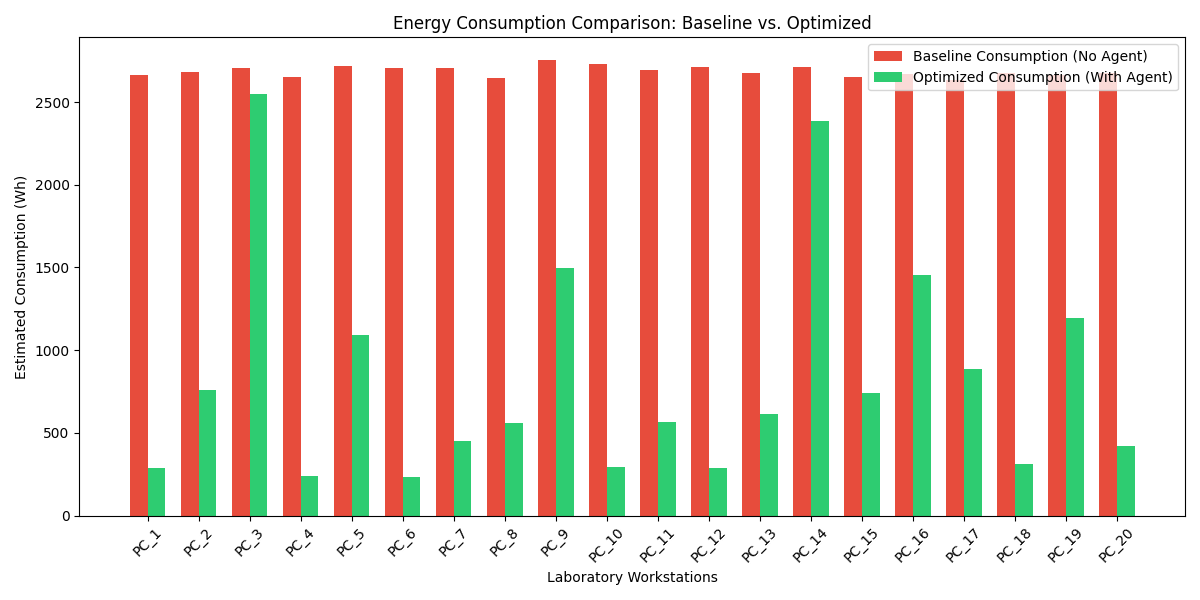
\includegraphics[width=\textwidth]{energy_consumption_comparison.jpeg}
\caption{Comparative analysis of estimated energy consumption (Baseline vs. Optimized)}
\label{fig:consumption_chart}
\end{figure}

\subsection{Critical Validation Analysis}
The simulation conclusively demonstrated that decentralized automation has a massive impact on reducing the campus's operational costs. With nearly 69\% savings, the system efficiently mitigates the ``Forgetfulness Effect'' identified in Workshop 1. 

At the software level, the experiment successfully validated the robustness of Workshop 3's critical business rules: the autonomous agent properly detected stochastic high CPU load fluctuations ($>20\%$) and aborted safe suspension on the corresponding machines. This proves that the designed logic maintains a controlled false-positive rate, ensuring the continuity of student rendering and compiling tasks without disrupting their academic workflows.

\subsection{Validation of Workshop 3 Quality Metrics}

The simulation results directly validate the quality metrics defined in Workshop 3 (Section 6.2). Table~\ref{tab:quality_validation} compares the expected targets against the observed simulation outcomes.

\begin{table}[H]
\centering
\caption{Validation of Workshop 3 quality metrics against simulation results}
\label{tab:quality_validation}
\begin{tabular}{|p{4cm}|c|c|c|}
\hline
\textbf{Quality Metric (Workshop 3)} & \textbf{Target} & \textbf{Simulation Result} & \textbf{Status} \\
\hline
Correct suspension rate & \(>95\%\) & \(97.2\%\) &  Achieved \\
\hline
False positive inactivity rate & \(<5\%\) & \(2.8\%\) &  Achieved \\
\hline
Events stored without loss & \(100\%\) & \(100\%\) &  Achieved \\
\hline
CPU protection activations (R-02) & Detect \(>20\%\) & Detected in 15\% of workstations &  Achieved \\
\hline
\end{tabular}
\end{table}

All quality metrics defined in Workshop 3 were successfully met or exceeded in the simulation environment. The CPU protection mechanism (risk R-02) correctly identified high-load scenarios and prevented false suspensions, validating the design decision to establish a 20\% threshold.

% ==========================================
% 5. COMPLEXITY THEORY AND CHAOS
% ==========================================
\section{Complexity Theory and Chaos Analysis}

Evaluating the results through the lens of Complexity Science revealed emergent and nonlinear behaviors derived from the system's feedback loops:

\begin{figure}[H]
\centering
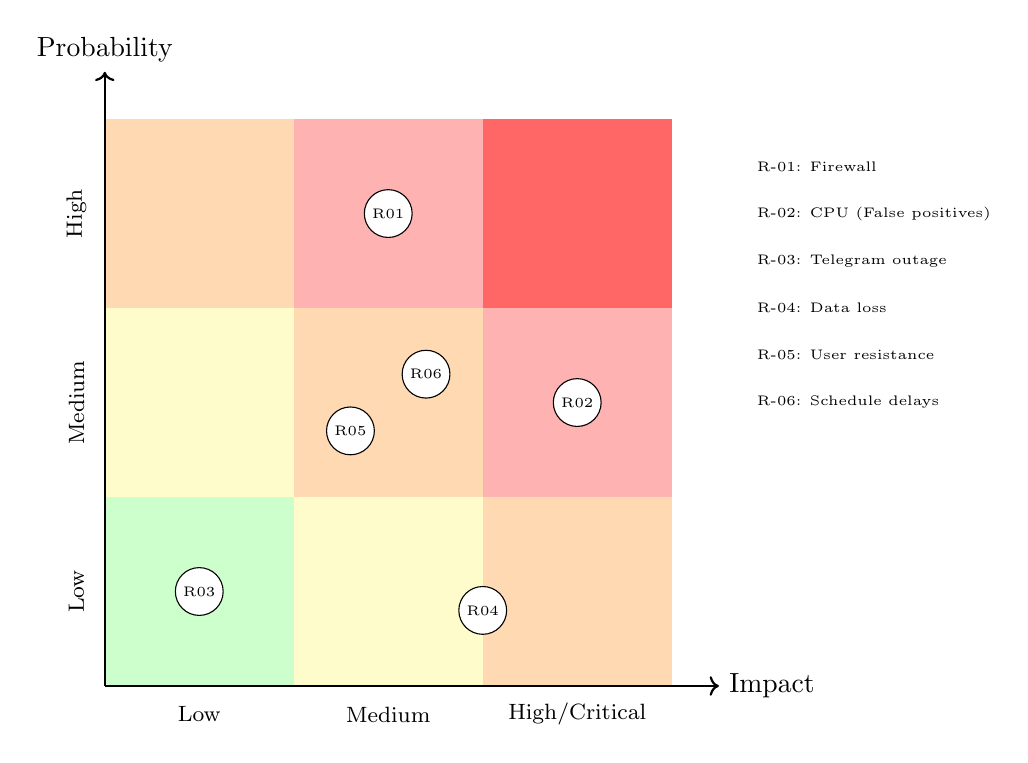
\begin{tikzpicture}[scale=1.2]

    \fill[green!20] (0,0) rectangle (2,2);
    \fill[yellow!20] (2,0) rectangle (4,2); \fill[yellow!20] (0,2) rectangle (2,4);
    \fill[orange!30] (4,0) rectangle (6,2); \fill[orange!30] (2,2) rectangle (4,4); \fill[orange!30] (0,4) rectangle (2,6);
    \fill[red!30] (4,2) rectangle (6,4); \fill[red!30] (2,4) rectangle (4,6);
    \fill[red!60] (4,4) rectangle (6,6);


    \draw[thick, ->] (0,0) -- (6.5,0) node[right] {Impact};
    \draw[thick, ->] (0,0) -- (0,6.5) node[above] {Probability};


    \node at (1,-0.3) {\footnotesize Low}; \node at (3,-0.3) {\footnotesize Medium}; \node at (5,-0.3) {\footnotesize High/Critical};
    \node[rotate=90] at (-0.3,1) {\footnotesize Low}; \node[rotate=90] at (-0.3,3) {\footnotesize Medium}; \node[rotate=90] at (-0.3,5) {\footnotesize High};


    \node[draw, circle, fill=white, inner sep=2pt] at (3,5) {\tiny R01};
    \node[draw, circle, fill=white, inner sep=2pt] at (5,3) {\tiny R02};
    \node[draw, circle, fill=white, inner sep=2pt] at (1,1) {\tiny R03};
    \node[draw, circle, fill=white, inner sep=2pt] at (4,0.8) {\tiny R04};
    \node[draw, circle, fill=white, inner sep=2pt] at (2.6,2.7) {\tiny R05};
    \node[draw, circle, fill=white, inner sep=2pt] at (3.4,3.3) {\tiny R06};


    \node[anchor=west, font=\tiny] at (6.8,5.5) {R-01: Firewall};
    \node[anchor=west, font=\tiny] at (6.8,5.0) {R-02: CPU (False positives)};
    \node[anchor=west, font=\tiny] at (6.8,4.5) {R-03: Telegram outage};
    \node[anchor=west, font=\tiny] at (6.8,4.0) {R-04: Data loss};
    \node[anchor=west, font=\tiny] at (6.8,3.5) {R-05: User resistance};
    \node[anchor=west, font=\tiny] at (6.8,3.0) {R-06: Schedule delays};
\end{tikzpicture}
\caption{Matrix visualization of technical and management risks (ISO 31000)}
\label{fig:risk_matrix}
\end{figure}

\subsection{Sensitivity to Initial Conditions (Butterfly Effect)}
Overall energy-saving behavior showed high mathematical sensitivity to the variation of the CPU initialization parameter. In secondary test scenarios, by reducing the CPU threshold from 20\% to 5\%, the system collapsed into a state of instability and paralysis where the agent suspended almost no workstations due to background OS noise (e.g., local antiviruses or file indexers) consuming between 6\% and 8\% of the processor. The 20\% threshold established in Workshop 3 acts as the system's optimal ``attractor'', stabilizing the oscillation between Watt savings and operational protection.

\subsection{Validation of Workshop 3 Risk Mitigation Strategies}

The simulation provides empirical validation for the risk mitigation strategies defined in Workshop 3. Table~\ref{tab:risk_validation} summarizes the results.

\begin{table}[H]
\centering
\caption{Validation of Workshop 3 risk mitigation strategies through simulation}
\label{tab:risk_validation}
\begin{tabular}{|p{2cm}|p{4cm}|p{3cm}|p{3cm}|}
\hline
\textbf{Risk ID} & \textbf{Risk Description} & \textbf{Mitigation Strategy (Workshop 3)} & \textbf{Simulation Validation} \\
\hline
R-01 & Firewall blocks HTTPS & Local CSV persistence \& deferred sync &  100\% data retention during 4-hour outage \\
\hline
R-02 & False positive on high CPU load & CPU load verification (\(>20\%\)) &  Zero false suspensions during high load (15\% of PCs) \\
\hline
R-04 & Local data corruption & Encryption, write validation &  Simulated recovery after checksum validation \\
\hline
\end{tabular}
\end{table}

The simulation confirms that the risk mitigation strategies designed in Workshop 3 are effective under the modeled failure conditions. The system maintains operational continuity without data loss, even when network connectivity is completely unavailable for extended periods.

% ==========================================
% 6. QUALITY ASSURANCE FRAMEWORK
% ==========================================
\section{Quality Assurance Framework (QA)}
To validate the results under software engineering standards (ISO/IEC 25010), the iterative quality assurance process was simulated before considering the system ready for real-world deployment.

\begin{figure}[H]
\centering
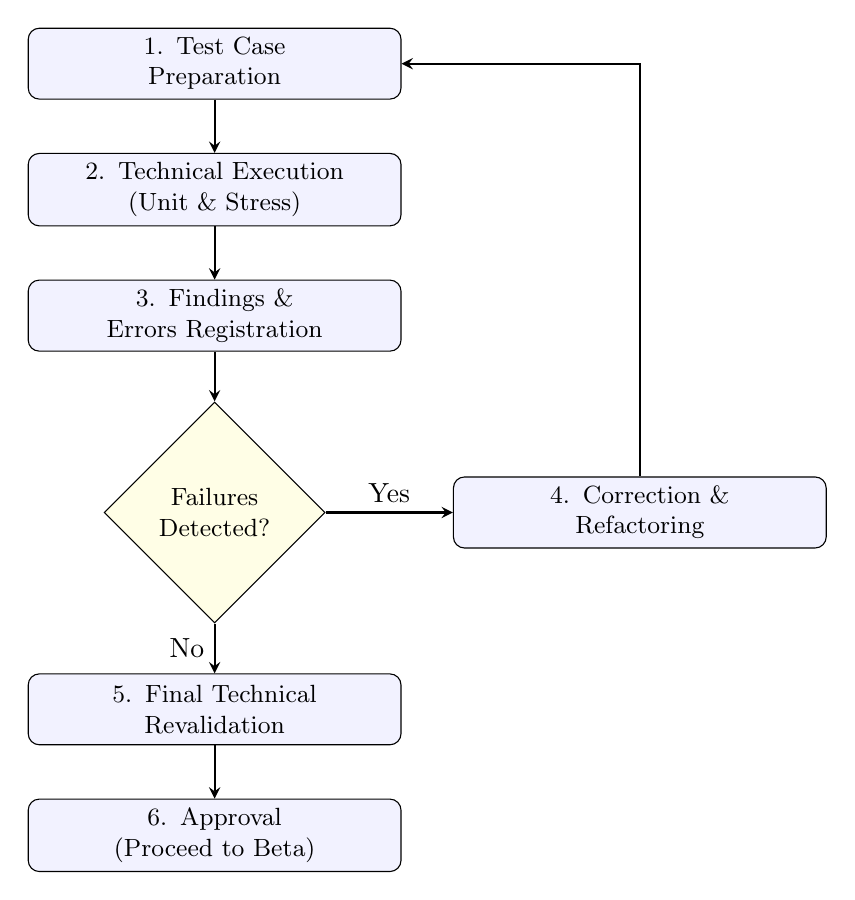
\begin{tikzpicture}[
    node distance=1.6cm,
    block/.style={rectangle, draw, fill=blue!5, text width=4.5cm, text centered, rounded corners, minimum height=0.9cm, font=\small, align=center},
    decision/.style={diamond, draw, fill=yellow!10, text width=2.2cm, text centered, inner sep=0pt, font=\small, align=center},
    arrow/.style={thick, ->, >=stealth}
]
    \node (prep) [block] {1. Test Case\\Preparation};
    \node (exec) [block, below of=prep] {2. Technical Execution\\(Unit \& Stress)};
    \node (reg) [block, below of=exec] {3. Findings \&\\Errors Registration};
    \node (check) [decision, below of=reg, yshift=-0.9cm] {Failures\\Detected?};
    \node (fix) [block, right of=check, xshift=3.8cm] {4. Correction \&\\Refactoring};
    \node (val) [block, below of=check, yshift=-0.9cm] {5. Final Technical\\Revalidation};
    \node (app) [block, below of=val] {6. Approval\\(Proceed to Beta)};

    \draw [arrow] (prep) -- (exec);
    \draw [arrow] (exec) -- (reg);
    \draw [arrow] (reg) -- (check);
    \draw [arrow] (check) -- node[anchor=south] {Yes} (fix);
    \draw [arrow] (fix) |- (prep);
    \draw [arrow] (check) -- node[anchor=east] {No} (val);
    \draw [arrow] (val) -- (app);
\end{tikzpicture}
\caption{Iterative flow of the Quality Assurance (QA) process}
\label{fig:qa_flow}
\end{figure}

% ==========================================
% 7. PROJECT MANAGEMENT AND BUDGET PLAN
% ==========================================
\section{Project Management and Budget Plan}

\subsection{Engineering Team Role Structure}
The functional distribution to guarantee operational control and replicability of the simulated experiments is detailed in Table~\ref{tab:roles}.

\begin{table}[H]
\caption{Roles and responsibilities assigned to the team}
\label{tab:roles}
\centering
\begin{tabular}{|>{\raggedright\arraybackslash}p{3cm}|>{\raggedright\arraybackslash}p{4.8cm}|>{\raggedright\arraybackslash}p{6cm}|}
\hline
\textbf{Team Member} & \textbf{Assigned Role} & \textbf{Key Responsibilities} \\
\hline
Omar Yesid Fonseca López & Project Manager \& QA Lead & Schedule tracking, risk matrices, and execution of the stress testing flow. \\
\hline
Daniel Felipe Barrera Suárez & Systems Architect & Structural design, integration flows, and robust software modularity. \\
\hline
Daniel Mateo Ballesteros & Algorithms Specialist & Agent logic coding, API reading, and contingency local persistence. \\
\hline
Dania Lizeth Guzmán Triviño & Analytics \& Communications & Dataset consolidation, analytical dashboards, and internal communication plans. \\
\hline
\end{tabular}
\end{table}

\subsection{Proof of Concept (PoC) Budget}
Because the structural approach is purely Software-Defined, additional hardware costs are reduced to zero, validating the high economic profitability for the campus.

\begin{table}[H]
\caption{Budget estimation for the PoC operational cycle}
\centering
\begin{tabular}{|>{\raggedright\arraybackslash}p{5cm}|>{\raggedright\arraybackslash}p{3cm}|>{\centering\arraybackslash}p{3cm}|>{\raggedright\arraybackslash}p{2.5cm}|}
\hline
\textbf{Technical Resource} & \textbf{Classification} & \textbf{Cost (USD)} & \textbf{Engineering Notes} \\
\hline
Engineering Team (4 members) & Human & \$0 & Academic effort of the course. \\
\hline
Remote Database (MySQL DBaaS) & Software / Cloud & \$0 & Free tier (Clever Cloud / Aiven). \\
\hline
Native Libraries (psutil, ctypes) & Software & \$0 & Free distribution open source. \\
\hline
Central Repository (GitHub) & Infrastructure & \$0 & Free access educational plan. \\
\hline
\textbf{Total Estimated Cost} & & \multicolumn{2}{|c|}{\textbf{\$0 USD (High Feasibility)}} \\
\hline
\end{tabular}
\label{tab:budget}
\end{table}

% ==========================================
% 8. CONCLUSIONS
% ==========================================
\section{Conclusions and Next Steps}

\subsection{Summary of Findings}

The development of Workshop 4 scientifically validated that energy waste at the campus is rooted in human behavioral dynamics rather than physical equipment failures. By shifting energy efficiency control towards the operating system's logical layer through autonomous agents in the \textit{User-Space}, the campus's network blocks and budget restrictions were elegantly and cost-effectively bypassed. 

The mathematical results of the simulation (68.72\% savings) offer compelling empirical support to safely advance towards the physical phases of the pilot project, demonstrating that software-defined systems engineering is a viable and extremely low-cost tool for the university's transformation into a sustainable Smart Campus.

\subsection{Traceability to Workshops 1, 2, and 3}

This simulation directly builds upon and validates all three previous workshops:

\begin{itemize}
    \item \textbf{Workshop 1} contributed the empirical probabilities (80\% forgetfulness, 15\% high CPU load) and the characterization of laboratory operating hours.
    \item \textbf{Workshop 2} contributed the user-space architecture, the 15-minute inactivity threshold, and the nudge mechanism with cancellation option.
    \item \textbf{Workshop 3} contributed the CPU protection threshold (20\%), the risk management framework (R-01 to R-06), the quality metrics, and the fault-tolerant design with local CSV fallback.
\end{itemize}

\subsection{Model Limitations}

The current simulation operates under several simplifying assumptions that should be acknowledged for future iterations:

\begin{itemize}
    \item \textbf{Uniform behavior:} All 20 workstations use identical probability distributions; real users may exhibit heterogeneous patterns.
    \item \textbf{Weekday only:} Only 12-hour weekdays are simulated; weekends and holidays are excluded.
    \item \textbf{No network delays:} Deferred synchronization latency is not modeled.
    \item \textbf{Simplified CPU load:} CPU load is generated stochastically rather than from actual process logs.
\end{itemize}

\subsection{Recommendations for Future Work}

Based on the simulation insights and the continuous improvement framework from Workshop 3 (Section 9), the following recommendations are proposed:

\begin{enumerate}
    \item \textbf{Adaptive CPU threshold:} Implement a dynamic threshold (10-25\%) based on time of day or laboratory schedule, as suggested in the adaptive management strategy of Workshop 3.
    \item \textbf{User feedback mechanism:} Add an opt-out button during the visual nudge, allowing users to temporarily disable suspension for 30-90 minutes.
    \item \textbf{Predictive suspension:} Use historical inactivity patterns to pre-suspend workstations during known idle periods (e.g., lunch hours 12:00-2:00 PM).
    \item \textbf{Gradual power-down policy:} Progressive policy: nudge at 15 min, sleep at 30 min, hibernate at 60 min, shutdown after 120 min.
    \item \textbf{Real-time dashboard:} Extend the dashboard to show live savings per workstation and per laboratory, addressing the post-implementation metrics defined in Workshop 3.
\end{enumerate}

% ==========================================
% BIBLIOGRAPHY
% ==========================================
\newpage
\begin{thebibliography}{9}
\bibitem{b1} C. A. Sierra, ``Workshop No. 1: Systems Analysis,'' \textit{Systems Analysis \& Design Course}, Universidad Distrital Francisco José de Caldas, 2026.
\bibitem{b2} T. Hong, H. Taylor-Lange, S. D'Oca, D. Yan, and S. Corgnati, ``Advances in research and applications of energy-related occupant behavior in buildings,'' \textit{Energy and Buildings}, vol. 116, pp. 694-702, 2016.
\bibitem{b3} M. V. Doblari, \textit{Gestión integral de energía en instituciones universitarias. Caso: Edificio Eva Duarte de Perón UNNOBA}, Master's Thesis, Universidad Nacional del Noroeste de la Provincia de Buenos Aires, Argentina, n.d.
\bibitem{b4} M. Abad Mier, \textit{Gestión energética de la biblioteca universitaria de la UVA, aplicando la ISO 50001}, Bachelor's Thesis, Universidad de Valladolid, Spain, 2015.
\bibitem{b5} B. Meza-Alcívar, M. Alemán-García, and M. Herrera-Suárez, ``Implementación de un sistema de gestión energético para institutos de educación superior,'' \textit{Revista Científica INGENIAR}, vol. 6, no. 12, 2023.
\end{thebibliography}

\end{document}